\documentclass[a4paper,12pt]{article}
\usepackage[utf8x]{inputenc}
\usepackage[swedish]{babel}
\usepackage[T1]{fontenc}
\usepackage{graphicx}
\usepackage{placeins}
\usepackage{bmpsize}
\usepackage{amsfonts, amsmath, amssymb}
\usepackage{ccfonts,euler}
\usepackage{wrapfig}
\usepackage{multirow}
\usepackage{caption}
\usepackage{enumerate}
\usepackage{comment}
\usepackage[includeheadfoot,margin=1.1in]{geometry}

\usepackage{listings}
\usepackage{listings}
\usepackage{color}

\definecolor{dkgreen}{rgb}{0,0.6,0}
\definecolor{gray}{rgb}{0.5,0.5,0.5}
\definecolor{mauve}{rgb}{0.58,0,0.82}

\lstset{frame=tb,
  language=Python,
  aboveskip=3mm,
  belowskip=3mm,
  showstringspaces=false,
  columns=flexible,
  basicstyle={\small\ttfamily},
  numbers=none,
  numberstyle=\tiny\color{gray},
  keywordstyle=\color{blue},
  commentstyle=\color{dkgreen},
  stringstyle=\color{mauve},
  escapeinside={\%*}{*)},
  breaklines=true,
  breakatwhitespace=true,
  tabsize=3,
  literate={å}{{\r a}}1 {ö}{{\"o}}1 {ä}{{\"a}}1 {Å}{{\r A}}1 {Ö}{{\"O}}1 {Ä}{{\"A}}1
}

\oddsidemargin -15mm
\evensidemargin -15mm
\marginparwidth 5mm
\topmargin -28mm
\textheight 282mm
\textwidth 190mm
\headheight 4mm
\headsep 4mm

\sloppy

\newcounter{iii}\setcounter{iii}{0}
\def\i{\bigskip\noindent\refstepcounter{iii}\textbf{\arabic{iii}.} }
%\def\iotst#1{\par \smallskip \mbox{}\refstepcounter{iii}\hspace*{#1}\textbf{\arabic{iii}.}}
\newcounter{pun}[iii]
\def\pu{\refstepcounter{pun}{\bf(\alph{pun})}\ }
\def\Pu{\par\noindent\mbox{}\refstepcounter{pun}{\phantom{\textbf{\arabic{iii}.}}\hspace{0.2mm}\bf(\alph{pun})}\ }

\def\ext{\subsection*{Extrauppgifter}}

\title{Programmering, Extraövningar}
\date{28 juli}

\makeatletter
\let\newtitle\@title
\let\newdate\@date
\makeatother
\begin{document}

  \renewcommand*\rmdefault{ppl}\normalfont\upshape
\pagestyle{empty}
\large
\section*{\newdate\ \  \newtitle}


\i Vad tror du att händer när koden körs? Fundera noga innan du testar att köra koden! Fundera sedan på varför du har rätt eller fel. 


\pu 
\begin{lstlisting}
>>> ['no', 'yes'][True]
\end{lstlisting}

\pu 
\begin{lstlisting}
>>> (0, 'a') < (1, 0)
>>> (1, 'a') < (1, 0)
\end{lstlisting}



\pu 
\begin{lstlisting}
>>> matrix = [[0] * 2] * 2
>>> matrix[0][0] = 1
>>> matrix
\end{lstlisting}


\pu 

\begin{lstlisting}
%*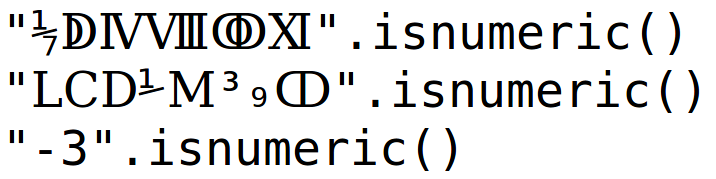
\includegraphics[width=0.3\textwidth]{kod}*)
\end{lstlisting}
Ni kan kopiera texten från www.technox.se/python\_oddity.html

\pu 
\begin{lstlisting}
>>> [1 if 2 else 3 for x4 in [5] if 6 if 7 if 8 if 9 or 0]
\end{lstlisting}

\pu % https://stackoverflow.com/questions/306313/is-operator-behaves-unexpectedly-with-integers
\begin{lstlisting}
>>> a = 256
>>> b = 256
>>> a is b
>>> a = 257
>>> b = 257
>>> a is b
>>> 257 is 257
\end{lstlisting}



\pu 
\begin{lstlisting}
>>> 5 in range(10) == True
\end{lstlisting}

\pu 
\begin{lstlisting}
>>> "hello" + True
>>> "hello" * True
\end{lstlisting}

\pu 
\begin{lstlisting}
>>> nums = reversed([1, 2, 3, 4]) 
>>> 2 in nums 
>>> 2 in nums
\end{lstlisting}
\newpage

\pu 
\begin{lstlisting}
>>> a = [1,2,3]
>>> b = {'a': 'b', 'c': 'd'}
>>> a += b
>>> a
\end{lstlisting}

\pu % https://dbader.org/blog/python-mystery-dict-expression
\begin{lstlisting}
>>> {True: 'yes', 1: 'no', 1.0: 'maybe'}
\end{lstlisting}


\pu
\begin{lstlisting}
d = {0}
for n, k in enumerate(d, 1):
    d.remove(k)
    d.add(n)
print(d)
\end{lstlisting}

\pu 
\begin{lstlisting}
>>> x, y = 999, 999
>>> x is y
>>> x = 999
>>> y = 999 
>>> x is y
\end{lstlisting}



\end{document}